\documentclass[tikz]{standalone}

\usepackage{tikz}
\usepackage{ensps-colorscheme}
%\usepackage{ifthen}

\usepackage{subcaption}

\pgfdeclarelayer{background}
\pgfsetlayers{background,main}

\begin{document}
	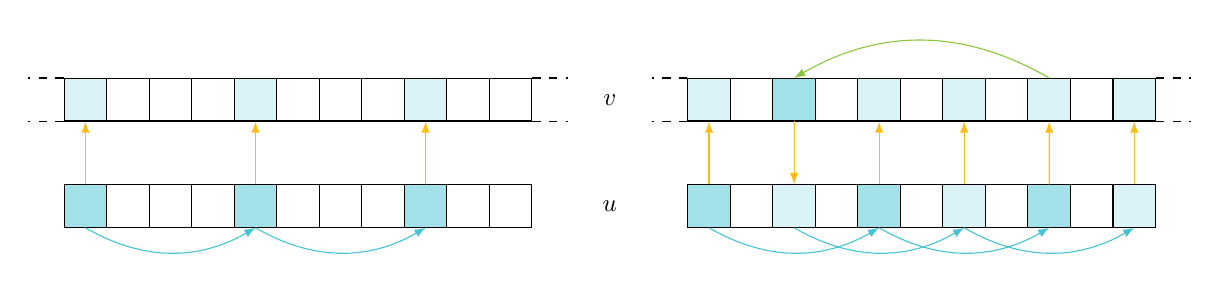
\begin{tikzpicture}[scale=0.9,every node/.style={scale=0.9}]
				
		\foreach \i in {1,...,11} {
			\pgfmathsetmacro{\x}{0.6 * \i}
			\node [draw,rectangle,minimum size=.6cm] (v\i) at (\x cm,0) {};
			\node [draw,rectangle,minimum size=.6cm] (u\i) at (\x cm,-1.5) {};
		}
		
		\node at (8cm,0) {$v$};
		\node at (8cm,-1.5) {$u$};
		
		
		\draw [dashed] (v1.north west) -- ++(-.5,0);
		\draw [dashed] (v1.south west) -- ++(-.5,0);		
		\draw [dashed] (v11.north east) -- ++(.5,0);
		\draw [dashed] (v11.south east) -- ++(.5,0);
		
		\path [color=D3,-{latex}] (u1) edge (v1);
		\path [color=D3,-{latex}] (u5) edge (v5);
		\path [color=D3,-{latex}] (u9) edge (v9);
		
		\path [color=D4,-{latex}] (u1.south) edge [bend right] (u5.south);
		\path [color=D4,-{latex}] (u5.south) edge [bend right] (u9.south);
		%\path [color=C5,-{latex}] (v9.north) edge [bend right] (v3.north);
		
		\begin{pgfonlayer}{background}
			\node [fill,color=D4bg,minimum size=.6cm] at (u1) {};
			\node [fill,color=D4bg,minimum size=.6cm] at (u5) {};
			\node [fill,color=D4bg,minimum size=.6cm] at (u9) {};
			\node [fill,color=D4hint,minimum size=.6cm] at (v1) {};
			\node [fill,color=D4hint,minimum size=.6cm] at (v5) {};
			\node [fill,color=D4hint,minimum size=.6cm] at (v9) {};	
		\end{pgfonlayer}
		
		
		\begin{scope}[shift={(8.8cm,0)}]
			\foreach \i in {1,...,11} {
				\pgfmathsetmacro{\x}{0.6 * \i}
				\node [draw,rectangle,minimum size=.6cm] (v\i) at (\x cm,0) {};
				\node [draw,rectangle,minimum size=.6cm] (u\i) at (\x cm,-1.5) {};
			}
			
			\draw [dashed] (v1.north west) -- ++(-.5,0);
			\draw [dashed] (v1.south west) -- ++(-.5,0);		
			\draw [dashed] (v11.north east) -- ++(.5,0);
			\draw [dashed] (v11.south east) -- ++(.5,0);
			
			\path [color=D3,-{latex}] (u1) edge (v1);
			\path [color=D3,-{latex}] (u5) edge (v5);
			\path [color=D3,-{latex}] (u9) edge (v9);
			
			\path [color=D3,-{latex}] (v3) edge (u3);
			\path [color=D3,-{latex}] (u7) edge (v7);
			\path [color=D3,-{latex}] (u11) edge (v11);
			
			\path [color=D4,-{latex}] (u1.south) edge [bend right] (u5.south);
			\path [color=D4,-{latex}] (u5.south) edge [bend right] (u9.south);
			
			\path [color=C5,-{latex}] (v9.north) edge [bend right] (v3.north);
			
			\path [color=D4,-{latex}] (u3.south) edge [bend right] (u7.south);
			\path [color=D4,-{latex}] (u7.south) edge [bend right] (u11.south);
	
			\begin{pgfonlayer}{background}
				\node [fill,color=D4bg,minimum size=.6cm] at (u1) {};
				\node [fill,color=D4bg,minimum size=.6cm] at (u5) {};
				\node [fill,color=D4bg,minimum size=.6cm] at (u9) {};
				\node [fill,color=D4hint,minimum size=.6cm] at (v1) {};
				\node [fill,color=D4hint,minimum size=.6cm] at (v5) {};
				\node [fill,color=D4hint,minimum size=.6cm] at (v9) {};	
				
				\node [fill,color=D4bg,minimum size=.6cm] at (v3) {};
				\node [fill,color=D4hint,minimum size=.6cm] at (u3) {};
				\node [fill,color=D4hint,minimum size=.6cm] at (v7) {};
				\node [fill,color=D4hint,minimum size=.6cm] at (u7) {};
				\node [fill,color=D4hint,minimum size=.6cm] at (v11) {};
				\node [fill,color=D4hint,minimum size=.6cm] at (u11) {};
			\end{pgfonlayer}
		\end{scope}
		
	\end{tikzpicture}
\end{document}
